\documentclass{beamer}

\pdfmapfile{+sansmathaccent.map}


\mode<presentation>
{
	\usetheme{Warsaw} % or try Darmstadt, Madrid, Warsaw, Rochester, CambridgeUS, ...
	\usecolortheme{seahorse} % or try seahorse, beaver, crane, wolverine, ...
	\usefonttheme{serif}  % or try serif, structurebold, ...
	\setbeamertemplate{navigation symbols}{}
	\setbeamertemplate{caption}[numbered]
} 


%%%%%%%%%%%%%%%%%%%%%%%%%%%%
% itemize settings

\definecolor{myhotpink}{RGB}{255, 80, 200}
\definecolor{mywarmpink}{RGB}{255, 60, 160}
\definecolor{mylightpink}{RGB}{255, 80, 200}
\definecolor{mypink}{RGB}{255, 30, 80}
\definecolor{mydarkpink}{RGB}{155, 25, 60}

\definecolor{mypaleblue}{RGB}{240, 240, 255}
\definecolor{mylightblue}{RGB}{120, 150, 255}
\definecolor{myblue}{RGB}{90, 90, 255}
\definecolor{mygblue}{RGB}{70, 110, 240}
\definecolor{mydarkblue}{RGB}{0, 0, 180}
\definecolor{myblackblue}{RGB}{40, 40, 120}

\definecolor{mygreen}{RGB}{0, 200, 0}
\definecolor{mygreen2}{RGB}{245, 255, 230}

\definecolor{mygray}{gray}{0.8}
\definecolor{mydarkgray}{RGB}{80, 80, 160}

\definecolor{mydarkred}{RGB}{160, 30, 30}
\definecolor{mylightred}{RGB}{255, 150, 150}
\definecolor{myred}{RGB}{200, 110, 110}
\definecolor{myblackred}{RGB}{120, 40, 40}

\definecolor{mygreen}{RGB}{0, 200, 0}
\definecolor{mygreen2}{RGB}{205, 255, 200}

\definecolor{mydarkcolor}{RGB}{60, 25, 155}
\definecolor{mylightcolor}{RGB}{130, 180, 250}

\setbeamertemplate{itemize items}[default]

\setbeamertemplate{itemize item}{\color{myblackblue}$\blacksquare$}
\setbeamertemplate{itemize subitem}{\color{mydarkblue}$\blacktriangleright$}
\setbeamertemplate{itemize subsubitem}{\color{mygray}$\blacksquare$}

\setbeamercolor{palette quaternary}{fg=white,bg=mygblue} %mydarkgray
\setbeamercolor{titlelike}{parent=palette quaternary}

\setbeamercolor{palette quaternary2}{fg=white,bg=mygblue}%black myblue
\setbeamercolor{frametitle}{parent=palette quaternary2}

\setbeamerfont{frametitle}{size=\Large,series=\scshape}
\setbeamerfont{framesubtitle}{size=\normalsize,series=\upshape}


%%%%%%%%%%%%%%%%%%%%%%%%%%%%
% block settings

%\setbeamercolor{block title}{bg=red!50,fg=black}
%\setbeamercolor{block title}{bg=mylightblue,fg=black}
\setbeamercolor{block title}{bg=myblackblue,fg=white}

\setbeamercolor*{block title example}{bg=mygreen!40!white,fg=black}

\setbeamercolor*{block body example}{fg= black,
	bg= mygreen2}


%%%%%%%%%%%%%%%%%%%%%%%%%%%%
% URL settings
\hypersetup{
	colorlinks=false,
	linkcolor=blue,
	filecolor=blue,      
	urlcolor=blue,
}

%%%%%%%%%%%%%%%%%%%%%%%%%%

\renewcommand{\familydefault}{\rmdefault}

\usepackage{amsmath}
\usepackage{mathtools}

\usepackage{subcaption}

\usepackage{qrcode}

\DeclareMathOperator*{\argmin}{arg\,min}
\newcommand{\bo}[1] {\mathbf{#1}}

\newcommand{\dx}[1] {\dot{\mathbf{#1}}}
\newcommand{\ma}[4] {\begin{bmatrix}
		#1 & #2 \\ #3 & #4
\end{bmatrix}}
\newcommand{\myvec}[2] {\begin{bmatrix}
		#1 \\ #2
\end{bmatrix}}
\newcommand{\myvecT}[2] {\begin{bmatrix}
		#1 & #2
\end{bmatrix}}

\newcommand{\R}{\mathbb{R}} 
\newcommand{\T}{^\top}     



\newcommand{\mydate}{Spring 2023}

\newcommand{\mygit}{\textcolor{blue}{\href{https://github.com/SergeiSa/Computational-Intelligence-Slides-Spring-2023}{github.com/SergeiSa/Computational-Intelligence-Slides-Spring-2023}}}

\newcommand{\myqr}{ \textcolor{black}{\qrcode[height=1.5in]{https://github.com/SergeiSa/Computational-Intelligence-Slides-Spring-2023}}
}

\newcommand{\myqrframe}{
	\begin{frame}
		\centerline{Lecture slides are available via Github, links are on Moodle}
		\bigskip
		\centerline{You can help improve these slides at:}
		\centerline{\mygit}
		\bigskip
		\myqr
	\end{frame}
}


\newcommand{\bref}[2] {\textcolor{blue}{\href{#1}{#2}}}



%%%%%%%%%%%%%%%%%%%%%%%%%%%%
% code settings

\usepackage{listings}
\usepackage{color}
% \definecolor{mygreen}{rgb}{0,0.6,0}
% \definecolor{mygray}{rgb}{0.5,0.5,0.5}
\definecolor{mymauve}{rgb}{0.58,0,0.82}
\lstset{ 
	backgroundcolor=\color{white},   % choose the background color; you must add \usepackage{color} or \usepackage{xcolor}; should come as last argument
	basicstyle=\footnotesize,        % the size of the fonts that are used for the code
	breakatwhitespace=false,         % sets if automatic breaks should only happen at whitespace
	breaklines=true,                 % sets automatic line breaking
	captionpos=b,                    % sets the caption-position to bottom
	commentstyle=\color{mygreen},    % comment style
	deletekeywords={...},            % if you want to delete keywords from the given language
	escapeinside={\%*}{*)},          % if you want to add LaTeX within your code
	extendedchars=true,              % lets you use non-ASCII characters; for 8-bits encodings only, does not work with UTF-8
	firstnumber=0000,                % start line enumeration with line 0000
	frame=single,	                   % adds a frame around the code
	keepspaces=true,                 % keeps spaces in text, useful for keeping indentation of code (possibly needs columns=flexible)
	keywordstyle=\color{blue},       % keyword style
	language=Octave,                 % the language of the code
	morekeywords={*,...},            % if you want to add more keywords to the set
	numbers=left,                    % where to put the line-numbers; possible values are (none, left, right)
	numbersep=5pt,                   % how far the line-numbers are from the code
	numberstyle=\tiny\color{mygray}, % the style that is used for the line-numbers
	rulecolor=\color{black},         % if not set, the frame-color may be changed on line-breaks within not-black text (e.g. comments (green here))
	showspaces=false,                % show spaces everywhere adding particular underscores; it overrides 'showstringspaces'
	showstringspaces=false,          % underline spaces within strings only
	showtabs=false,                  % show tabs within strings adding particular underscores
	stepnumber=2,                    % the step between two line-numbers. If it's 1, each line will be numbered
	stringstyle=\color{mymauve},     % string literal style
	tabsize=2,	                   % sets default tabsize to 2 spaces
	title=\lstname                   % show the filename of files included with \lstinputlisting; also try caption instead of title
}

%%%%%%%%%%%%%%%%%%%%%%%%%%%%
% tikz settings

\usepackage{tikz}
\tikzset{every picture/.style={line width=0.75pt}}

%%%%%%%%%%%%%%%%%%%%%%%%%%%%




\title{Interior Point Method}
\subtitle{Computational Intelligence, Lecture 14}
\author{by Sergei Savin}
\centering
\date{\mydate}



\begin{document}
\maketitle


\begin{frame}{Content}

\begin{itemize}
	\item Newton method
	\item Barrier functions
	\item Interior point method
	\item Analytic center of linear inequalities
%\item Lagrange dual function
%\item Duality gap, strong and weak duality
%\item Sensitivity
%\item Homework
\end{itemize}

\end{frame}





\begin{frame}{Newton method, 1}
	% \framesubtitle{General form}
	\begin{flushleft}
		
		Given a function $f: \R \rightarrow \R$, we can write it as $y = f(x)$. Consider the problem of finding roots of the equation $f(x) = 0$.
		
		\bigskip
		
		To solve it we can use an iterative procedure. We start at the initial guess $x_0$, produce affine approximation of the function at this point using constant and linear terms of its Taylor expansion:
		
		\begin{equation}
			f = f(x_0) + \frac{\partial f}{\partial x} (x - x_0) + \text{h.o.t.},
		\end{equation}
		
		and then solve the problem $f(x_0) + \frac{\partial f}{\partial x} (x - x_0) = 0$, to find a new point $x_1$, which will serve the role of $x_0$ during the next iteration. This is called \emph{Newton's method}.
		
	\end{flushleft}
\end{frame}


\begin{frame}{Newton method, 2}
	% \framesubtitle{General form}
	\begin{flushleft}
		
		The solution to the equation $f(x_0) + \frac{\partial f}{\partial x} (x - x_0) = 0$ is:
		
		\begin{equation}
			x = x_0  - \left ( \frac{\partial f}{\partial x} \right )^{-1} f(x_0)
		\end{equation}
		
		% TODO: \usepackage{graphicx} required
		\begin{figure}
			\centering
			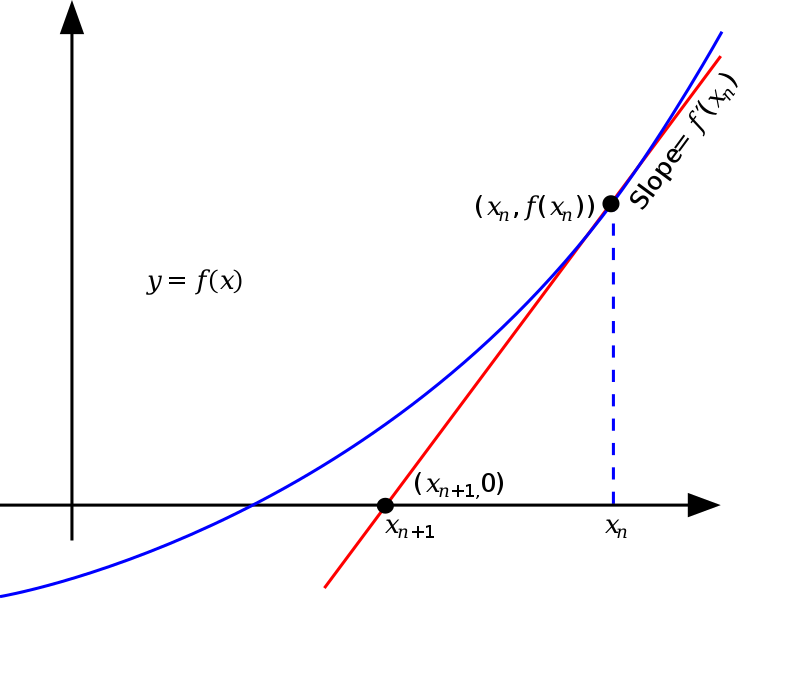
\includegraphics[width=0.6\linewidth]{Newton_iteration}
			\label{fig:newtoniteration}
		\end{figure}
		
		
	\end{flushleft}
\end{frame}



\begin{frame}{Sequantial quadratic approximation, 1}
	% \framesubtitle{General form}
	\begin{flushleft}
		
		Given a function $\varphi: \R \rightarrow \R$, we can write it as $y = \varphi(x)$. Let us find minimum of this function.
		
		\bigskip
		
		We can try to do it by looking at its quadratic approximation (considering constant, linear and quadratic terms of the Taylor expansion) at an approximation point $x_0$:
		
		\begin{equation}
			\varphi = \varphi(x_0) + \frac{\partial \varphi}{\partial x} (x - x_0)
			+ \frac{1}{2} (x - x_0) \frac{\partial^2 \varphi}{\partial x^2} (x - x_0)
			 + \text{h.o.t.},
		\end{equation}
		%
		and finding its minimum, which can be done by solving a single least-squares problem. Its solution $x_1$ becomes the next approximation point.
		
		\bigskip
		
		This is \emph{another form of the Newton's method}, and is completely equivalent to the previously discussed one. 
		
		
		
	\end{flushleft}
\end{frame}




\begin{frame}{Sequantial quadratic approximation, 2}
	% \framesubtitle{General form}
	\begin{flushleft}
		
		Let us define $g =\left. \frac{\partial \varphi}{\partial x} \right \vert_{x = x_0}$ and $H = \left. \frac{\partial^2 \varphi}{\partial x^2}\right \vert_{x = x_0}$. Let us solve the problem:
		
		\begin{equation}
			\text{minimize:} \ \ \varphi(x_0) + g (x - x_0)
			+  \frac{1}{2}  (x - x_0) H (x - x_0)
		\end{equation}
		
		The minimum is attained when the derivative is achieves zero:
		
		\begin{equation}
			g + (x - x_0) H = 0
		\end{equation}
		
		This gives us solution $x = x_0 - H^{-1} g$.
		
	\end{flushleft}
\end{frame}





\begin{frame}{Connection of two methods}
	% \framesubtitle{General form}
	\begin{flushleft}
		
		Let us define a function $p(x) = \frac{\partial \varphi}{\partial x}$. Function $\varphi (x)$ achieves minimum when $p(x)$ crosses zero. Solving the problem $p(x) = 0$ with Newton's method, we initiate iterative process:
		
		\begin{equation}
			x_{i+1} = x_i  - \left ( \frac{\partial p}{\partial x} \right )^{-1} p(x_i)
		\end{equation}
		
		Given the definition of $p(x)$ we can re-write this expression as:
		
		\begin{equation}
			x_{i+1} = x_i  - \left ( \frac{\partial^2 \varphi}{\partial x^2} \right )^{-1} \frac{\partial \varphi}{\partial x}
		\end{equation}
		
		Using previously defined variables $g =\frac{\partial \varphi}{\partial x}$ and $H = \frac{\partial^2 \varphi}{\partial x^2}$ we obtain the same expression we saw in sequatial quadratic approximation:
		%
		\begin{equation}
			x_{i+1} = x_i  - H^{-1} g
		\end{equation}

	\end{flushleft}
\end{frame}





\begin{frame}{Multivariable Newton's method}
	% \framesubtitle{General form}
	\begin{flushleft}
		
		For mutivaribe case $\varphi: \R^n \rightarrow \R$ the Taylor expansion is given exactly the same:
		%
		\begin{equation}
			\varphi = \varphi(\bo{x}_0) + \frac{\partial \varphi}{\partial \bo{x}} (\bo{x} - \bo{x}_0)
			+ \frac{1}{2} (\bo{x} - \bo{x}_0) \frac{\partial^2 \varphi}{\partial \bo{x}^2} (\bo{x} - \bo{x}_0)
			+ \text{h.o.t.},
		\end{equation}
		
		Solution to the quadratic approxamation is given as:
		
		\begin{align}
			\bo{x}_{i+1} &= \bo{x}_i  - \bo{H}^{-1} \bo{g}
			\\
			\bo{x}_{i+1} &= \bo{x}_i  - \left(\frac{\partial^2 \varphi}{\partial \bo{x}^2} \right)^{-1} 
													 \frac{\partial \varphi}{\partial \bo{x}} 
		\end{align}
		
		A key feature of Neuton's method is very fast convergence near the solution.
		
	\end{flushleft}
\end{frame}






\begin{frame}{Solving constrained optimization}
	% \framesubtitle{General form}
	\begin{flushleft}
		
		Newton's method works for \emph{unconstrained optimization}.
		
		\bigskip
		
		Linear equalities in convex programs can often be excluded by introducing new variables in the null space of the constraints.
		
		\bigskip
		
		Inequality constraints can be replaces with \emph{soft constraints} - an addition to the cost function which punishes decision variables that approach the border of the domain. 
		
	\end{flushleft}
\end{frame}



\begin{frame}{Linear inequalities}
% \framesubtitle{General form}
\begin{flushleft}

Consider linear inequality constraints:

\begin{equation}
    \bo{A}\bo{x} \leq \bo{b}
\end{equation}

Remember that we can rewrite it as:

\begin{equation}
    \bo{a}_i^\top \bo{x} \leq b_i
\end{equation}
\begin{equation}
\label{eq:linear_constraints}
    \bo{a}_i^\top \bo{x} - b_i \leq 0
\end{equation}

Instead of \emph{hard constraints} in \eqref{eq:linear_constraints} we can turn these into a cost function component:

\begin{equation}
    J = -\sum\limits_{i = 1}^n \text{log} (b_i - \bo{a}_i^\top \bo{x})
\end{equation}

Which is called a \emph{barrier function}.
 
\end{flushleft}
\end{frame}




\begin{frame}{Barrier functions}
% \framesubtitle{General form}
\begin{flushleft}

Let us consider barrier functions $J = -\sum\limits_{i = 1}^n \text{log} (b_i - \bo{a}_i^\top \bo{x})$:

\begin{itemize}
    \item It removes the constraint, but modifies the cost.
    \item When $b_i - \bo{a}_i^\top \bo{x}$ is a very small positive number, $\text{log} (b_i - \bo{a}_i^\top \bo{x})$ is a very big negative number, hence the minus sign in front.
    \item Barrier function does not behave well outside of the domain, when $b_i - \bo{a}_i^\top \bo{x} < 0$.
\end{itemize}
 
\end{flushleft}
\end{frame}




\begin{frame}{Barrier functions for QPs}
% \framesubtitle{General form}
\begin{flushleft}

Hence the following QP:

\begin{equation}
\begin{aligned}
& \underset{\bo{x}}{\text{minimize}}
& & \bo{x}^\top \bo{H} \bo{x} + \bo{f}^\top \bo{x}, \\
& \text{subject to}
& & 
\bo{A}\bo{x} \leq \bo{b}
\end{aligned}
\end{equation}
 
...can be approximated as:

\begin{equation}
\begin{aligned}
& \underset{\bo{x}}{\text{minimize}}
& & \bo{x}^\top \bo{H} \bo{x} + \bo{f}^\top \bo{x} - \sum\limits_{i = 1}^n \text{log} (b_i - \bo{a}_i^\top \bo{x})
\end{aligned}
\end{equation}
 
\end{flushleft}
\end{frame}





\begin{frame}{Zero-infinity barrier function}
	% \framesubtitle{General form}
	\begin{flushleft}
		
		Zero-infinity function can be seen as a precise barrier - adding nothing to teh cost in the domain interior and punishing constraint violation by infinite increase of cost:
		
		\begin{equation}
		f(x) = 
		\begin{cases}
			0 &x \leq 0 \\
			\infty &x > 0
		\end{cases}
		\end{equation}
		
		This can be written as max over a family of linear functions:
		
		\begin{equation}
			f(x) = 
			\underset{\lambda \geq 0}{\text{max}}  \  \lambda x
		\end{equation}		
		
		The QP discussed in the previous example becomes:
		
		\begin{equation}
			\begin{aligned}
				& \underset{\bo{x}}{\text{minimize}} \ \underset{\lambda \geq 0}{\text{max}}
				& & \bo{x}^\top \bo{H} \bo{x} + \bo{f}^\top \bo{x} - \sum\limits_{i = 1}^n \lambda_i (b_i - \bo{a}_i^\top \bo{x})
			\end{aligned}
		\end{equation}
		
		It appears that we re-discovered Lagrangian method.
		
		
	\end{flushleft}
\end{frame}




\begin{frame}{Interior point method, 1}
	% \framesubtitle{General form}
	\begin{flushleft}
		
		Interior point method is based on KKT conditions with a single modification highlifgted below:
		
		\begin{enumerate}
			\item Lagrangian stationarity: $\frac{\partial f_0(\bo{x}) }{\partial \bo{x}} 
			+
			\sum\limits_i 
			\lambda_i  \frac{\partial g_i(\bo{x}) }{\partial \bo{x}} 
			= 0$.
			
			\item Primal feasibility: $g_i(\bo{x}) \leq 0$.
			
			\item Dual feasibility: $\lambda_i \geq 0$.
			
			\item Complementarity slackness: $\lambda_i g_i(\bo{x}) = \textcolor{red}{-\bo{t}_i}$.
		\end{enumerate}
		
		\bigskip
		
		From the complementarity we can find expression for lagrange multipliers:
		
		\begin{equation}
			\lambda_i = -\frac{t_i}{g_i(\bo{x})}
		\end{equation}
		
	\end{flushleft}
\end{frame}




\begin{frame}{Interior point method, 2}
	% \framesubtitle{General form}
	\begin{flushleft}
		
		Given $\lambda_i = -\frac{t_i}{g_i(\bo{x})}$ we can transform the Lagrangian stationarity condition:
		%
		\begin{equation}
			\frac{\partial f_0(\bo{x})}{\partial \bo{x}} 
			-
			\sum\limits_i 
			\frac{t_i}{g_i(\bo{x})}
			\frac{\partial g_i(\bo{x})}{\partial \bo{x}} 
			= 0
		\end{equation}
		
		Let us compute the following derivative:
		%
		\begin{align}
			\frac{\partial}{\partial \bo{x}} (  -t \log ( -g(\bo{x}) )  ) 
			= \frac{-t}{-g(\bo{x})} (-1) \frac{\partial g(\bo{x})}{\partial \bo{x}} 
			= -\frac{t}{g(\bo{x})} \frac{\partial g(\bo{x})}{\partial \bo{x}} 
		\end{align}
		
		With that, we can re-write the lagrangain conndition:
		%
		\begin{equation}
			\frac{\partial f_0(\bo{x})}{\partial \bo{x}} 
			-
			\frac{\partial}{\partial \bo{x}} 
			\left(
			\sum\limits_i 
			t_i \log (- g_i (\bo{x})) 
			\right) = 0
		\end{equation}
		
		
	\end{flushleft}
\end{frame}



\begin{frame}{Interior point method, 3}
	% \framesubtitle{General form}
	\begin{flushleft}
		
		Condition $\frac{\partial f_0(\bo{x})}{\partial \bo{x}} 
		-
		\frac{\partial}{\partial \bo{x}} 
		\left(
		\sum\limits_i 
		t_i \log (- g_i (\bo{x})) 
		\right) = 0$ is equivalent to minimization:
		
		
		\begin{equation}
			\label{KKT_to_opt}
			\begin{aligned}
				& \underset{\bo{x}}{\text{minimize}}
				& & f_0(\bo{x}) - 
				\sum\limits_i t_i \log (- g_i (\bo{x})) 
			\end{aligned}
		\end{equation}
		
		Solution to this problem $\bo{x}^*$ implies that $\log (- g_i (\bo{x}))$ exists, meaning that $g_i (\bo{x}) \leq 0$, giving us primal feasibility.
		
		\bigskip
		
		In the same way, $\lambda_i = -\frac{t_i}{g_i(\bo{x})} \geq 0$, giving us dual feasibility.
		
		\bigskip
		
		Thus, we have all KKT conditions satisfied automatically by solving the minimization \eqref{KKT_to_opt}.
		
	\end{flushleft}
\end{frame}



\begin{frame}{Interior point method. Central path}
	% \framesubtitle{General form}
	\begin{flushleft}
		
		\emph{Interior point method} consists of constructing problem \eqref{KKT_to_opt} and solving it using Newton's method for a given value of $t_i$; the method is applied iteratively, with dwindling $t_i$ over subsequent iterations. Solution $\bo{x}^*$ of the previous iteration is used to initialize Newton's method on the next iteration.
		
		\bigskip
		
		The sequence of $\bo{x}^*$ resulting from this iterative process iis called \emph{central path}. 
		
		\bigskip
		
		As $t_i$ approaches zero, the log barriers $t_i \log (- g_i (\bo{x}))$ show less and less influence on the position of the optimzal solution, allowing us to approximate the solution to the original problem more and more accurately.
		
	\end{flushleft}
\end{frame}





\begin{frame}{Analytic center of linear inequalities}
% \framesubtitle{General form}
\begin{flushleft}

We can define \emph{analytic center of linear inequalities} as a minimum of the function $J = -\sum\limits_{i = 1}^n \text{log} (b_i - \bo{a}_i^\top \bo{x})$. And that can be solved as a convex optimization:

\begin{align*}
    \bo{x}_a = \underset{\bo{x}}{\text{argmin}} & \ \  -\sum\limits_{i = 1}^n \text{log} (b_i - \bo{a}_i^\top \bo{x})
\end{align*}

At the analytic center of linear inequalities the shape of contour lines can be analysed as a local quadratic approximation of the function $J$:

\begin{equation}
    \mathcal{C} = \{ \bo{x}: \ (\bo{x} - \bo{x}_a)^\top \frac{\partial^2 J}{\partial \bo{x}^2} (\bo{x} - \bo{x}_a) = \epsilon \}
\end{equation}

where $\epsilon$ is a small number.
  
\end{flushleft}
\end{frame}



\begin{frame}{Illustration of a barrier functions}
% \framesubtitle{Parameter estimation}
\begin{flushleft}

\begin{figure}
    \centering
    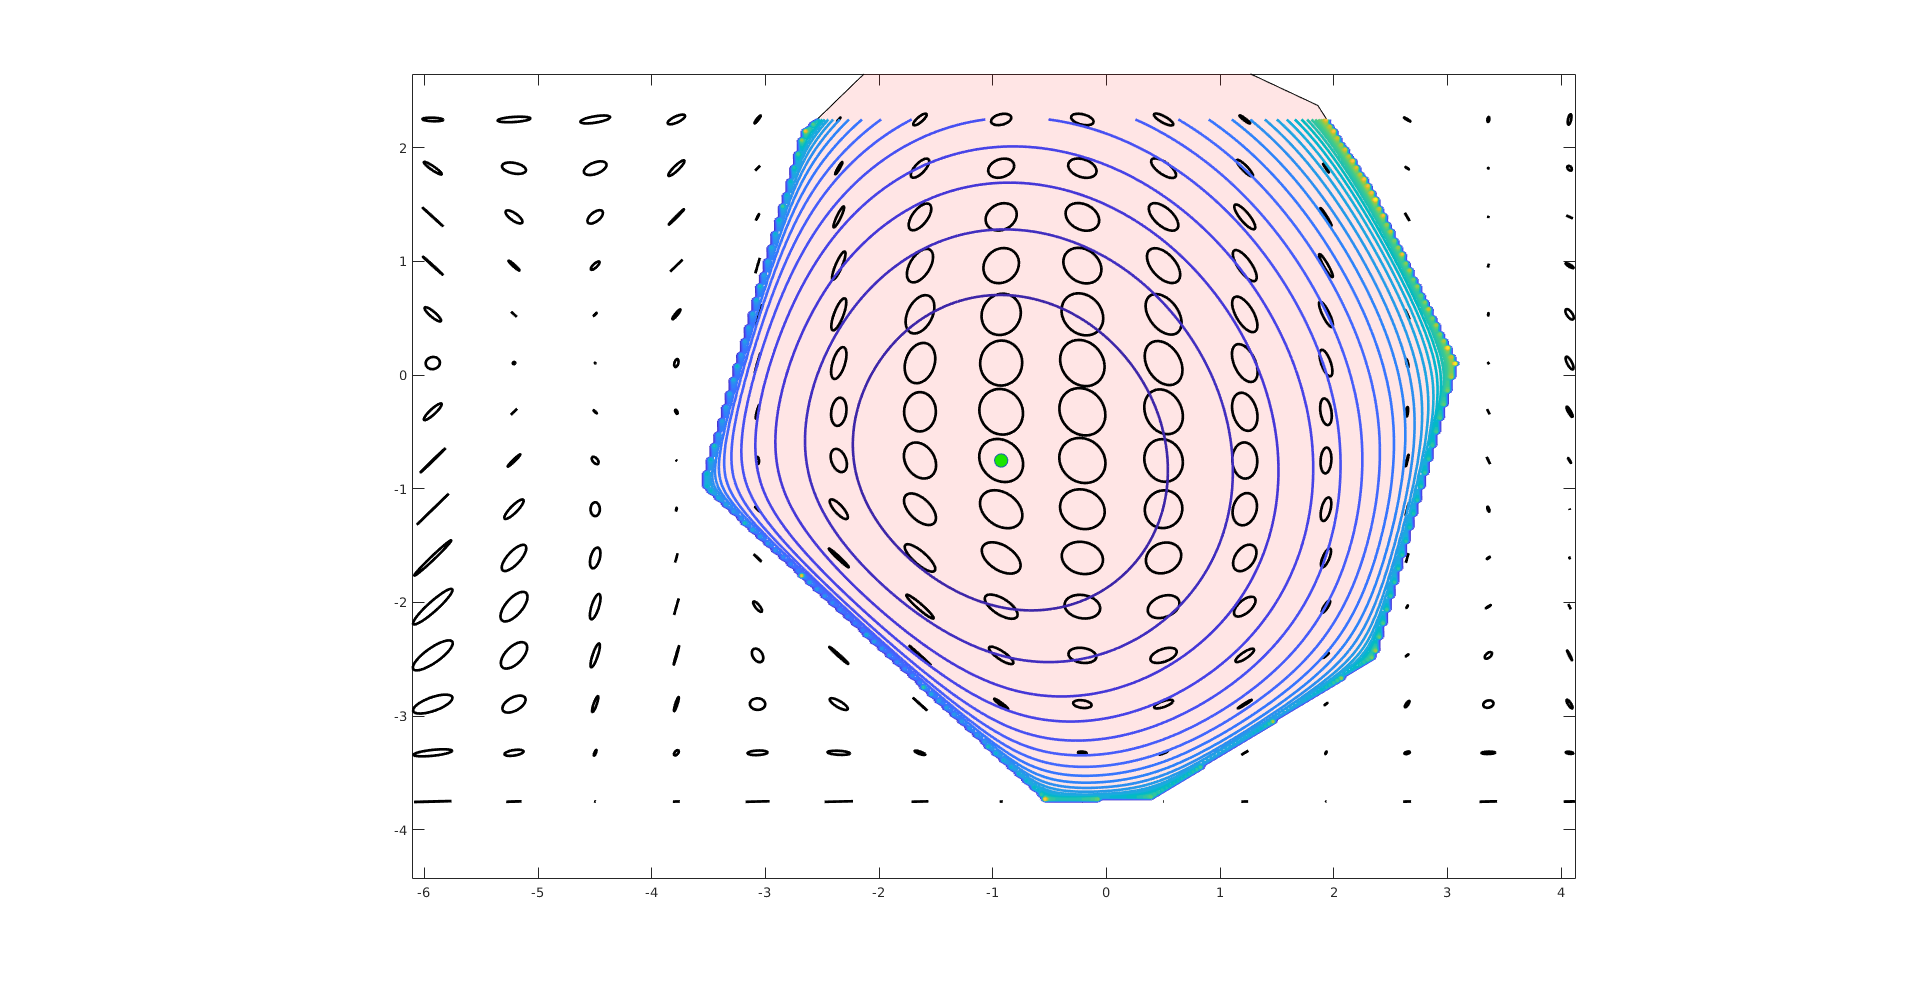
\includegraphics[width=\linewidth]{LogBarrier2.png}
    %\caption{Domain}
    \label{fig:BarrierFunctions}
\end{figure}

Pink is the domain. The ellipsoids represent the shape of the hessian $\frac{\partial^2 J}{\partial \bo{x}^2}$ at different points on the domain. Green dot is $\bo{x}_a$.

\end{flushleft}
\end{frame}







%\begin{frame}{Homework}
%% \framesubtitle{Parameter estimation}
%\begin{flushleft}
%
%Visualize contours of a quadratic program of your choice. Compute its optimal lower bound and duality gap.
%
%\end{flushleft}
%\end{frame}



\myqrframe



\end{document}
